
\section{First Member}
This is the section dedicated to one of the team members, and it should be written individually . It can include a range of things; first subsection is a space for you to point out the strengths and weaknesses of the module, including complaints about the module coordinator Max Wilson. The second section should have a selfie image with Max! The last part of it is the most important one. You will need to write a paragraph about what you have learned in this module. You can write it in \textbf{Bold} if you want or you can use other fonts. 

Please do not forget:
\begin{itemize}
	\item First paragraph should have your comments about the module
	\item Second one, a selfie img with Max
	\item Last one, what you learned in this module.
\end{itemize}

\subsection{Comments about the module}

Well, the module has happened, isn't that great, we have the ability to remember a whole bunch of \textbf{bunches} of diagram types, \textbf{bought} a book for the expected reading to find out that all of the expected reading was provided with the sources of these documents looking \textbf{less legitimate} each passing week. But the labs, for the \textbf{labs} and the teamwork it has all been worth it.

The best part of the module has been the \textbf{labs} I have actually \textbf{enjoyed} working with my {fabulous} team. 

\subsection{Selfie with Max}

To include an image, you will need to remove the comments from the code below, place an image in the main folder, and do not forget to put the name of the image instead of ImgName. 


\begin{figure}[h]
\caption{Selfie with Max, inspired by Julian}
\centering
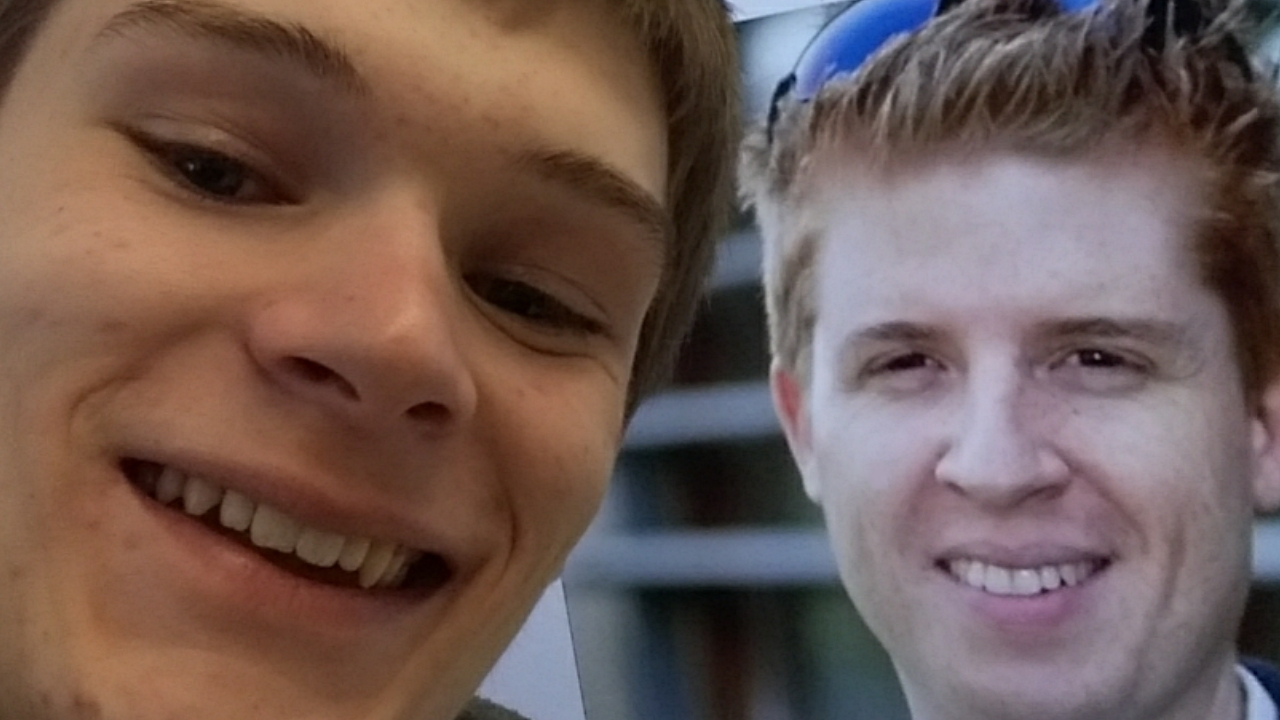
\includegraphics[width=1.0\textwidth]{maxSelfieJoshua.jpg}
\label{fig:selfie}
\end{figure}

You can then use the label of the figure to reference it later with the command ${\backslash}ref$. you can comment out the next line to see an example of how it works.

My selfie with Max is in  Figure~\ref{fig:selfie}.

\subsection{What I have learned in this module}

Teamwork makes the \textbf{dream} work. It is completely vital to plan to save development costs. You really need to talk to your clients, find out the requirements, make a specification, do low and high level planning. Create prototypes, liaise with the clients all of the way. then when you are sure that all of the specification is done, you plan the tests. Then you can finally start coding. All that is left is to do testing, first internally, then acceptance and user testing. Done!

\subsection{What I have learned today}

\textbf{Don't let team members submit stuff without first testing that it actually works!}
\textbf{Just because there is no work for a member does not mean that they have not done the work}